% ICRA draft: robot ultrasound bladder monitoring for HoLEP morcellation.
%
% Format follows the IEEEtran two-column conference style of the reference PDF
% (~/Downloads/main.pdf): Times New Roman text and math, anonymous submission,
% figure captions that open with a bold lead phrase.
%
% House rules applied here: no em dashes anywhere in the text, and every glyph
% set in Times New Roman (newtxtext + newtxmath).
%
% Figure policy: four real figures are wired in from figures/ (console capture,
% force rig, stiffness measurement, final setup). The three that still have to be
% drawn reserve vertical space and carry their caption, with \includegraphics
% commented out.
%
% That is seven figures, which is more than a six page ICRA body will hold. The
% cheapest cuts, in order: fold the console capture into the overview figure as
% one panel, and drop the pipeline diagram in favour of text.
%
% Every number below is traceable to this repository. Items marked \TODO are
% not measured yet, or are pending the closed-loop runs.
\documentclass[conference]{IEEEtran}
\IEEEoverridecommandlockouts

\usepackage{newtxtext}   % Times New Roman text
\usepackage{newtxmath}   % Times New Roman math
\usepackage{amsmath,amssymb}
\usepackage{graphicx}
\usepackage{booktabs}
\usepackage{siunitx}
\usepackage{xcolor}
\usepackage{balance}
\usepackage[hidelinks]{hyperref}

\sisetup{detect-all}
\newcommand{\TODO}[1]{\textcolor{red}{\textbf{[TODO: #1]}}}
\newcommand{\figspace}[1]{\vspace{#1}}

\begin{document}

\title{Keeping the Bladder in View: A Force Regulated Ultrasound Robot for HoLEP
Morcellation Trained on Probe Mounted Demonstrations Without Robot Data}

\author{Anonymous Authors\thanks{Blind for review. Anonymous Authors are with
Anonymous Institution.}}

\maketitle

\begin{abstract}
During the morcellation phase of holmium laser enucleation of the prostate
(HoLEP), an assistant holds a suprapubic ultrasound probe for the length of the
phase so that the surgeon can watch bladder filling and volume. The task is
monotonous but not trivial: the probe must stay coupled at a safe force while
the bladder changes shape and volume underneath it. We present an ultrasound
robot that takes over this monitoring task, and a demonstration pipeline that
trains it without ever moving the robot to collect data. Contact force is
measured by a Hall effect force/torque sensor between the flange and the probe.
Against a laboratory scale over \SIrange{0.92}{9.85}{\newton} the compensated
reading is linear with slope \num{1.019} (95\% CI \numrange{0.975}{1.064},
$R^2=\num{0.993}$), and an admittance loop holds a commanded contact force to
\SI{0.028}{\newton} standard deviation across eight set points from
\SIrange{0.5}{4.0}{\newton} on a torso mannequin holding an air tube that a
syringe inflates and deflates. Demonstrations are recorded by instrumenting the clinical
probe itself with a six axis inertial sensor: the sonographer scans by hand,
and probe rotation is recovered at \SI{2.50}{\degree} geodesic RMS against robot
forward kinematics, five times better than the on chip nine axis fusion near
the robot (\SI{11.23}{\degree} axial RMS). The two streams are joined on one
host clock after removing a measured \SI{200}{\milli\second} effective image
latency. A U-Net segments the bladder lumen (Dice \num{0.874} on bladder present
held out frames) and feeds two separate quality functions: $Q_\mathrm{seg}$,
the learning objective, which scores whether the bladder is seen, large and
laterally centred, and $Q_\mathrm{raw}$, a segmentation independent image score
that drives an extremum seeking search over the contact force set point. On
\num{4389} demonstration chunks we train an ACT style conditional VAE that
predicts \SI{1.6}{\second} action chunks and ranks candidate chunks by a
predicted future quality head. \TODO{closed loop policy result on the dynamic
bladder phantom}. We also report a negative result that constrains this class
of method: on freehand demonstrations the quality head learns motion magnitude
but not motion direction (mirror test \SI{52.4}{\percent}, chance
\SI{50}{\percent}), so candidate ranking collapses onto a single elevational
direction in \SI{84}{\percent} of held out observations.
\end{abstract}

\section{Introduction}

Holmium laser enucleation of the prostate is performed under continuous
irrigation, and during morcellation the bladder must stay adequately filled but
never over distended. Standard practice is for an assistant to hold a suprapubic
ultrasound probe over the bladder for the duration of the phase so that the
operating surgeon can judge filling and volume~\cite{jang2024selftraining,trinkler2019bladder}. The work is static, long, and
delegated to a person whose clinical judgement is spent on holding a probe
still; and because the assistant tires, the view drifts at the moment the
surgeon needs it.

This paper asks whether that monitoring task can be handed to a robot without
also handing over the clinical judgement. Our answer is a system built around
two loops that are physically separable: a contact loop that keeps the probe
pressed within a verified force envelope, and an image loop that keeps the
bladder in the picture. Everything above those two loops stays with the
clinician.

The obstacle is not control but data. Learning a probe motion policy from
demonstrations normally requires the demonstrations to be collected on the
robot, and in an operating room that is precisely what cannot be done. Our
second contribution is therefore a demonstration route that never involves the
robot: the sonographer's own probe carries an inertial sensor, the ultrasound
stream is captured in parallel, and the pair is turned into observation and
action chunks after the fact. The robot appears only as the ground truth used to
validate the sensor, and later as the executor.

Our contributions are:

\begin{enumerate}
\item \textbf{A force regulated ultrasound probing stack}
(Sec.~\ref{sec:system}): a Hall effect force/torque sensor between the FR5
flange and a wireless convex probe, attitude dependent gravity compensation
validated against a laboratory scale, an admittance loop that owns the beam
axis, and a safety envelope of \SI{3}{\newton} target, \SI{4.5}{\newton}
warning and \SI{5}{\newton} forced retreat, verified under repeated volume
disturbances.
\item \textbf{Robot free demonstration capture} (Sec.~\ref{sec:data}): probe
mounted six axis inertial sensing with a measured image to inertial latency,
stillness bracketed action chunks, and a characterisation of what such labels
can and cannot support, namely rotation yes and translation no.
\item \textbf{Two quality functions with different jobs}
(Sec.~\ref{sec:percep}): a segmentation based score that defines the learning
objective, and a segmentation independent score that defines the contact force
set point, so that ``press harder'' and ``look elsewhere'' never compete for the
same signal. Because the freehand demonstrations carry no force channel, the
force axis cannot be imitated and is instead searched online.
\item \textbf{An image conditioned action chunk policy}
(Sec.~\ref{sec:policy}) with a predicted quality head for candidate selection,
evaluated against pre-registered hold and placebo controls on a dynamic bladder
phantom (Sec.~\ref{sec:exp}), together with an analysis of why the learned
quality head cannot yet supply direction (Sec.~\ref{sec:negative}).
\end{enumerate}

We do not claim autonomy of the clinical task. The robot is a probe holder that
keeps a view; the decisions that follow from the view remain the surgeon's.

\begin{figure}[t]
\centering
% \includegraphics[width=\linewidth]{fig1_overview.pdf}
\figspace{34mm}
\caption{\textbf{From the sonographer's hand to the robot's.} (a) Demonstration
capture: the clinical probe carries a six axis inertial sensor, and ultrasound
and inertial data are joined on one host clock. (b) The robot: FR5 arm, Hall
effect force/torque sensor, wireless convex probe. (c) Closed loop operation on
the dynamic bladder phantom, with the force loop on the beam axis and the policy
on the rotational axes.}
\label{fig:overview}
\end{figure}

\section{Related Work}

\textbf{Robotic ultrasound.} Robotic ultrasound systems and their control
strategies are surveyed
in~\cite{priester2013robotic,vonhaxthausen2021medical,li2021overview,jiang2023robotic}.
Force is usually handled either by a hybrid force and position controller for
freehand assisted scanning~\cite{gilbertson2015force} or by pressing along a
planned trajectory registered to a preoperative volume~\cite{hennersperger2017towards},
and the closest analogue to an image driven objective is confidence driven
servoing, which steers the probe by an ultrasound confidence
map~\cite{chatelain2017confidence}. Existing systems therefore either servo
towards a target view learned from robot collected sweeps, or press with a fixed
force profile. Our setting differs
in both respects: the demonstrations come from a hand held clinical probe, and
the force set point is not fixed but searched online against image quality.

\textbf{Demonstration collection without a robot.} Learning from demonstration
normally assumes the demonstration is recorded on the
learner~\cite{argall2009survey,ravichandar2020recent}; hand held capture devices
break that assumption by instrumenting the tool
instead~\cite{chi2024umi}. Recovering probe motion from a hand held ultrasound
probe is an old problem in freehand 3D reconstruction, solved with external
trackers, with speckle decorrelation~\cite{prager1999stradx,housden2007sensorless}
or, more recently, learned from the images
themselves~\cite{prevost2018freehand}. The medical variant of the problem is
that the instrument belongs to the clinician, not the robot. In our case the instrument is the ultrasound probe itself, and the signal
that must survive the transfer is probe orientation rather than gripper pose.

\textbf{Action chunking and imitation.} We build on ACT style action chunking
with a conditional VAE~\cite{zhao2023act}, and add a quality head that scores the
future image consequence of a candidate chunk. That head is what is meant to
turn replay into selection, and Sec.~\ref{sec:negative} reports how far it
actually gets on freehand data.

\textbf{Bladder segmentation and ultrasound image quality.} Bladder
segmentation from ultrasound is well covered, from wall segmentation
networks~\cite{saini2026bwsnet} to compute constrained models for handheld
bladder monitors~\cite{song2023memory}, and reinforcement learning has been
used to guide a bladder scan towards a better view~\cite{hsu2026active}. Our
perception stage follows the standard U-Net recipe~\cite{ronneberger2015unet},
pretrained on a public pelvic floor
corpus~\cite{solismartin2026pfus1,garciamejido2024applicability}. The contribution here is not the network but the
physical gating that deletes predictions where no measurement exists, and the
separation of the two quality functions.

\section{System}
\label{sec:system}

\subsection{Hardware}

A Fairino FR5 six axis arm carries, in series from the flange, a PX6D Hall
effect six axis force/torque sensor, a printed mount, and a Konted C10UR
wireless convex ultrasound probe. The mount places the probe axis at
\SI{43}{\degree} to the flange plane with a \SI{199}{\milli\metre} lever arm,
and the probe assembly mass is \SI{231}{\gram}. The probe streams $160$ A-lines
by $512$ depth samples as \texttt{uint8}, before scan conversion, at
\SIrange{9.98}{10.4}{\hertz} over its own Wi-Fi access point. Differential
inverse kinematics runs at \SI{100}{\hertz}, the joint servo at
\SI{125}{\hertz}, and the force/torque sensor streams at \SI{1}{\kilo\hertz}.

\subsection{Force measurement and gravity compensation}

The sensor sits proximal to a heavy, off axis tool, so the raw wrench is
dominated by the tool's own weight, which rotates with the arm; before
compensation the beam axis component moves by about \SI{\pm 8}{\newton} with
attitude. Mass, centre of mass and mounting angle are identified from a
19 pose sweep (identified mass \SI{200}{\gram}, fit residual
\SI{0.152}{\newton}), and constraining the fit to the single physical stack axis
reduces the residual from \SI{0.183}{\newton} to \SI{0.047}{\newton} on the same
data. Only the compensated wrench is published to the control stack.

Over 19 unloaded poses the compensation residual is
\SI{0.000\pm0.182}{\newton} (mean $\pm$ SD, RMSE \SI{0.177}{\newton}, maximum
\SI{0.376}{\newton}). The residual is not white: its rank correlation with pose
index is $\rho = +0.896$ ($p < \num{1e-4}$), that is, a systematic attitude
dependent term rather than noise. We therefore do not subtract it. In deployment
the constant part is removed by a working pose tare taken immediately before
each run, and what remains bounds the accuracy of the force loop. Sensor noise
is \SI{\pm 0.05}{\newton} per axis at the configured dead band, and
\SI{0.015}{\newton} standard deviation at \SI{1}{\kilo\hertz}.

\subsection{Validation against a laboratory scale}

To check that the compensated reading is the contact force and not an artefact
of the compensation, the mounted probe was pressed onto a laboratory scale
(resolution \SI{1}{\gram}, standard uncertainty \SI{0.0028}{\newton}) at loads
from \SI{0.92}{\newton} to \SI{9.85}{\newton}; 19 of 20 trials were analysed.
Regressing the robot reading on the scale reference gives slope \num{1.019}
(95\% CI \numrange{0.975}{1.064}), intercept \SI{-0.373}{\newton} (95\% CI
\numrange{-0.587}{-0.158}) and $R^2 = \num{0.99269}$. Bland and Altman analysis
gives a bias of \SI{-0.293}{\newton} with 95\% limits of agreement
\numrange{-0.734}{+0.148}\,\si{\newton}; mean absolute error is
\SI{0.344}{\newton}, which is \SI{3.49}{\percent} of the \SI{9.85}{\newton} full
scale. In other words the \emph{scale factor} is correct to within
\SI{2}{\percent} while a sub newton offset remains, of the same order as the
attitude dependent compensation residual. We report the offset rather than
calibrating it away: a fixed offset correction was implemented and then removed,
because it is not constant across attitudes and would hide the residual it
partially cancels.


\begin{figure*}[t]
\centering
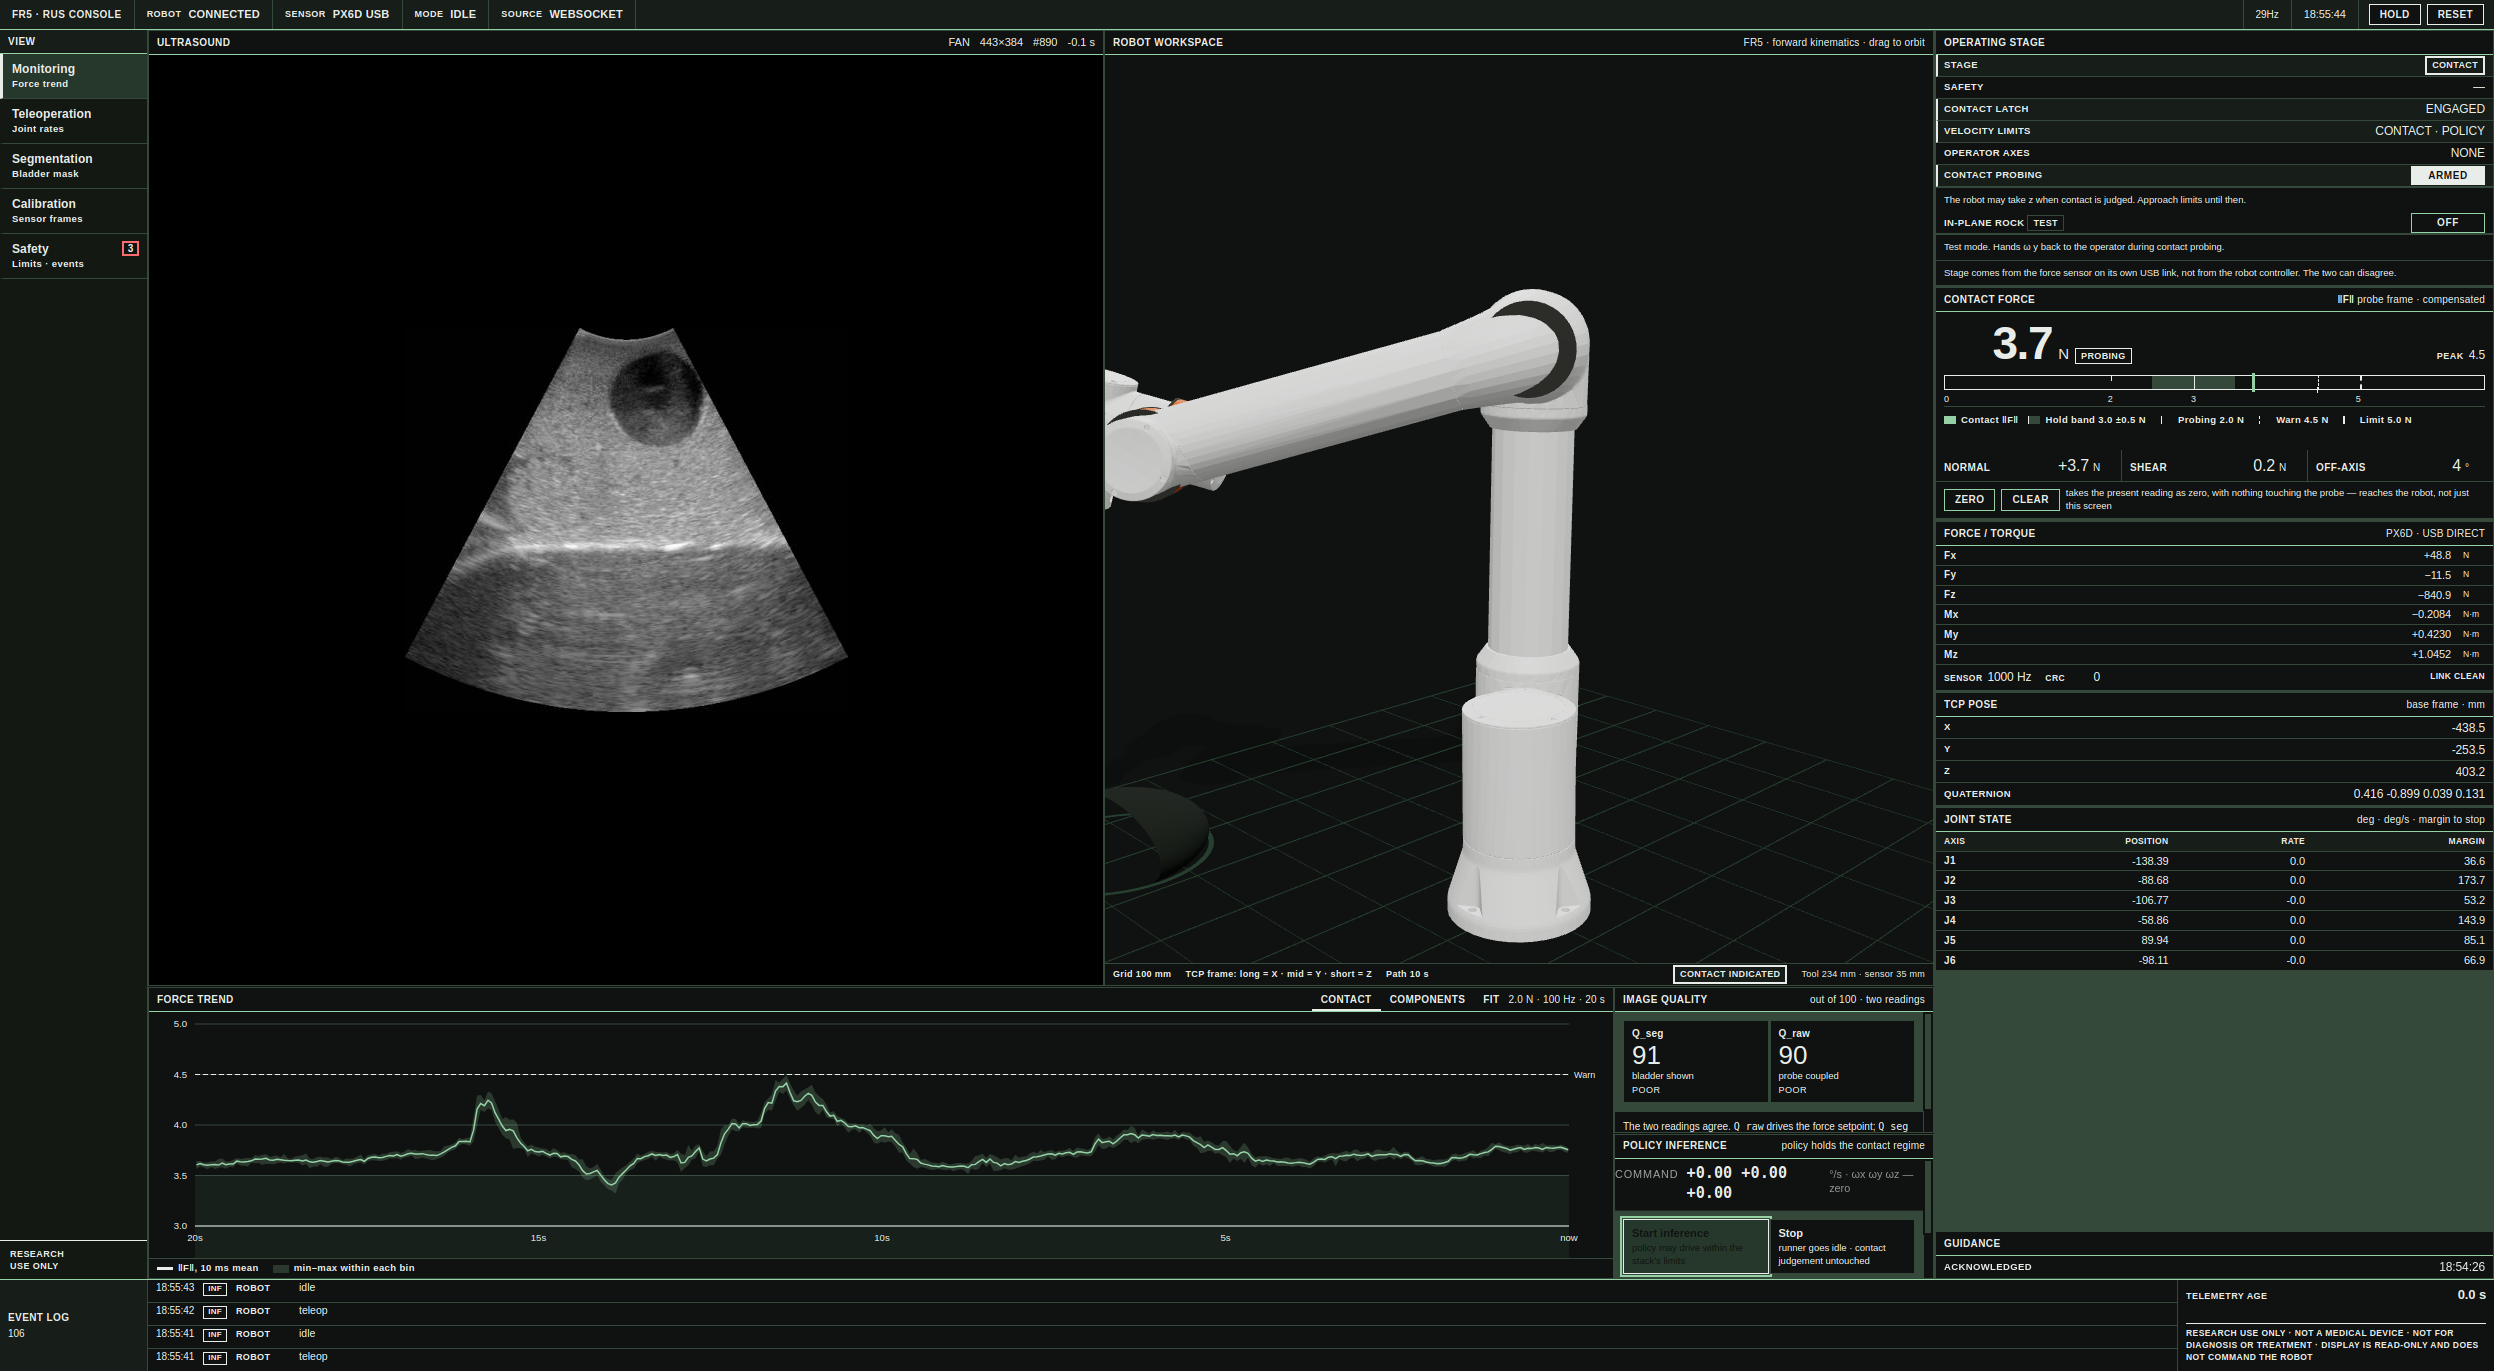
\includegraphics[width=\textwidth]{figures/console_bladder.png}
\caption{\textbf{The operator console during a policy episode.} Left: the live
sector image with the bladder in view. Centre: the arm in its own workspace, and
below it the contact force trend against the hold band and the warning line.
Right: the declared regime and the contact force with its bands, and at the
bottom the two quality readings, $Q_\mathrm{seg}$ and $Q_\mathrm{raw}$, beside
the policy panel that starts and stops inference and shows the commanded
angular rates. The console reads and displays; it issues no motion of its own
beyond the two buttons.}
\label{fig:console}
\end{figure*}

\subsection{Contact regulation and the safety envelope}

The beam axis $z$ is owned by an admittance regulator, never by the operator and
never by the policy:
\begin{equation}
v_z = \frac{F^\star - F_n}{B_z},\qquad |v_z| \le v_{\max},
\end{equation}
with $B_z = \SI{4500}{\newton\second\per\metre}$, a dead band of
\SI{0.05}{\newton} about $F^\star$, and a retreat speed of
\SI{5}{\milli\metre\per\second}. The dead band and gain were chosen together:
at $B_z = \num{1000}$ and \num{3000} the loop limit cycles with a period of
\SIrange{8}{9}{\second} and a force amplitude of \SI{\pm 0.35}{\newton}, because
the measured contact stiffness of the phantom rises from
\SI{0.28}{\newton\per\milli\metre} at \SI{0.5}{\newton} to
\SI{1.8}{\newton\per\milli\metre} at \SI{4}{\newton} while the force lags
indentation by \SIrange{1.5}{2.4}{\second}. At $B_z = \num{4500}$ the loop gain
falls to \numrange{0.01}{0.20} over that stiffness range and the limit cycle
disappears, at the cost of a slow response: the time constant is
$B_z/k \approx \SI{12}{\second}$ for the measured phantom stiffness
$k = \SI{0.374}{\newton\per\milli\metre}$.

Three limits are enforced above the regulator: a hold target of
\SI{3}{\newton}, a soft warning at \SI{4.5}{\newton} at which rising commands
are refused, and a hard limit of \SI{5}{\newton} at which the regulator
overrides everything and retreats along $-z$ until the force falls below
\SI{0.2}{\newton}. A two layer watchdog retreats the probe if twist commands
stop for \SI{100}{\milli\second} and stops the joints if joint commands stop for
the same interval. Velocity limits are switched by regime:
\SI{150}{\milli\metre\per\second} in free space,
\SI{10}{\milli\metre\per\second} and \SI{0.2}{\radian\per\second} once the
contact regime is entered.

\section{Demonstrations Without a Robot}
\label{sec:data}

\subsection{Instrumented probe and synchronisation}

A BNO085 inertial measurement unit on a Seeed XIAO nRF52840 Sense is clamped to
the probe in a printed split shell. Accelerometer and gyroscope report at
\SI{200}{\hertz} each and the on chip rotation vector at \SI{100}{\hertz}; the
host runs a magnetometer free gradient descent attitude
filter~\cite{madgwick2011estimation} and logs \SIrange{250}{256}{\hertz} of CRC
protected records over USB serial,
keeping both device and host timestamps. The ultrasound stream and the inertial
stream share exactly one clock, the host's reception time.

Reception time is not acquisition time. We measure the fixed delay of the
ultrasound path by cross correlating frame to frame image change with the box
integrated gyroscope magnitude over the same interval,
\begin{equation}
\hat\tau_{us} = \arg\max_{\tau}\ \operatorname{corr}\!\big(\Delta I_i,\ \Omega_i(\tau)\big),
\end{equation}
and obtain $\hat\tau_{us} = \SI{200}{\milli\second}$ pooled over 268 sessions
($r = \num{0.817}$, session bootstrap 95\% CI
\numrange{190}{200}\,\si{\milli\second}, and injected artificial delays are
recovered with \SI{0}{\milli\second} error). This is an \emph{effective} latency
that includes the scanner's frame persistence rather than a transport delay
specification. It is subtracted once, in the dataset builder.

\subsection{Six axes, not nine}

Near a moving steel arm, magnetometer aided fusion is not merely noisier, it is
wrong. We characterise the sensor on a bench in which the instrumented probe is
held by the robot, so that forward kinematics supplies ground truth over an
\SI{83.8}{\second} teleoperated block of probing rhythm (\num{16757} paired
samples). The bench probe is a clamped clinical convex probe in a printed split
shell; the phantom demonstrations reported below were captured with a second,
wireless probe in the same manner, so the orientation figures characterise the
sensing route rather than one specific clamp. Against that ground truth, host
side six axis fusion gives per channel rotation RMS of \SI{1.14}{\degree}, \SI{0.73}{\degree}
and \SI{1.95}{\degree} (tilt $x$, tilt $y$, axial), geodesic RMS
\SI{2.50}{\degree} (p95 \SI{3.56}{\degree}), static alignment residual
\SI{0.81}{\degree} and axial drift \SI{0.23}{\degree\per\minute}. The on chip
nine axis rotation vector, on the same recordings, gives \SI{11.23}{\degree}
axial RMS, \SI{6.68}{\degree} alignment residual and
\SI{8.29}{\degree\per\minute} drift (Table~\ref{tab:imu}). The cause is
positional rather than attitudinal: a pose paired magnetic test near the robot
found no usable stationary pairs at all, and a sensor fixed distortion model
leaves residuals up to \num{9.6} times the noise with direction errors up to
\SI{56.8}{\degree}. A field that changes with \emph{where} the probe is cannot
be calibrated out by any attitude model, which is the failure mode reported for
motion laboratories~\cite{devries2009magnetic,sabatini2011estimating}, so we
disable the magnetometer, give up
absolute heading, and claim only rotation relative to a session reference pose.
Against our own pre-registered limit of \SI{2.0}{\degree} the geodesic RMS of
\SI{2.50}{\degree} is a fail, and we report it as one; every other criterion
(alignment, latency, correlation, drift, displacement floor) passes.

Translation is the counter example. With zero velocity bracketing the
displacement error floor is \SI{0.25}{\milli\metre} at \SI{0.5}{\second} and
\SI{6.32}{\milli\metre} at \SI{5}{\second}, against \SI{12.4}{\milli\metre} and
\SI{1236.5}{\milli\metre} for raw double integration; over 21 real move
segments the error is one to two orders of magnitude above that floor. On 65
elevational sweep segments of the demonstration set, the drift removed by the
zero velocity bracket has a median of \SI{60}{\milli\metre} against a median
net displacement of \SI{14}{\milli\metre}, a ratio of \num{2.75}. Translation
is kept in the dataset for completeness and is never commanded.

\subsection{Sensor to probe rotation}

The inertial sensor is clamped in an arbitrary attitude. We rotate the probe
about each of its own axes in a dedicated session and take the principal axis of
the gyroscope samples, the first right singular vector, as the corresponding row
of $R_{SP}$. The recovered axes are mutually \SI{93.2}{\degree},
\SI{92.7}{\degree} and \SI{97.7}{\degree} apart with a \SI{4.20}{\degree}
projection residual and $\det R_{SP} = \num{+1.000}$, and a gravity check fixes
the beam axis sign. Axis assignment is unambiguous, with off diagonal terms
below \num{0.024}. The \emph{signs} of the lateral and elevational rows are
not: an independent argument from the demonstration data, in which the sign of
the starting acceleration agrees with the direction of image structure motion in
146 of 146 lateral translation sessions, yields the opposite sign to the
rotation session above. Both candidates have determinant $+1$, so this is a
convention difference rather than a mounting difference, and it stays open
(Sec.~\ref{sec:limits}).

\subsection{From freehand scanning to action chunks}

Freehand scanning is not continuous: the sonographer moves, holds, and moves
again. We detect stillness from gyroscope and accelerometer statistics in a
\SI{0.30}{\second} window and take each still to still interval as one move
segment, accepting durations from \SI{0.15}{\second} to \SI{8.0}{\second}. The
median still fraction is \SI{54.2}{\percent} and \SI{82}{\percent} of intervals
are accepted. Within a segment, rotation comes from the fused rotation vector
and translation from doubly integrated linear acceleration with a zero end
velocity de-drift, the bracketing idea that pedestrian inertial navigation uses
between footfalls~\cite{foxlin2005pedestrian,skog2010zerovelocity}.

The dataset is 268 sessions and \num{45902} frames, comprising a continuous
scanning day (20 sessions, \num{19708} frames) and a search task (248 episodes,
\num{26194} frames) in which each episode begins with the bladder out of view.
Total recording time is \SI{77}{\minute}. It yields \num{1818} move segments
and \num{4389} observation and action chunks, split by session (218 train, 26
validation, 24 test) into \num{3297}, \num{576} and \num{516} chunks.
Each observation is $m = 20$ frames at $256^2$ with a 21 dimensional perception
state per frame and a 15 dimensional scalar vector; each action label is a
$k = 8$ step chunk of \SI{1.6}{\second} at \SI{5}{\hertz}. All demonstrations
come from one bladder phantom and one operator, so the validation and test
splits measure reproducibility on that phantom, not generalisation.


\section{Perception and the Two Quality Functions}
\label{sec:percep}

\subsection{Scan conversion and contact measurement}

Polar frames are converted to a sector B-mode image with the vendor geometry
(radius \SI{59}{\milli\metre}, half angle \SI{28}{\degree}, depth
\SI{220}{\milli\metre}), giving \SI{0.443}{\milli\metre} per pixel and a
$512 \times 591$ grid that is letterboxed to $256^2$. The same converter runs in
training and at run time.

In freehand capture the probe is often only partially coupled, and near field
brightness cannot decide coupling because transducer ring down is bright in air
as well (mid depth mean: 6 in air against 55 in contact). We call an A-line
coupled when its mid depth mean exceeds a threshold, and define the frame
contact ratio $\rho$ as the fraction of coupled lines. Over \num{45902} frames,
\SI{70.0}{\percent} of continuous scanning frames are fully coupled
($\rho \ge \num{0.90}$) against \SI{43.8}{\percent} of search episode frames, and
$\rho$ predicts segmentation accuracy monotonically.

\subsection{Bladder segmentation}

A standard U-Net (\num{8.6}\,M parameters, \SI{16.3}{\giga MAC} at $256^2$),
pretrained on a public pelvic floor ultrasound corpus of 110 patients and
\num{14852} annotated frames, is fine tuned on the phantom with 234 human drawn
labels collected over six active learning rounds. Inference takes
\SI{1.1}{\milli\second} per frame and the full perception chain, including the
control features, \SI{3.0}{\milli\second} on an RTX 4090, against a runtime
budget of \SI{125}{\milli\second} set by the observation window. The acquisition function ranks frames by boundary entropy and
neighbour frame mask IoU, which correlate with per frame Dice
($r = \num{-0.636}$ and $r = \num{+0.694}$), whereas a threshold free confidence
score does not ($r = \num{+0.507}$, and degenerate at \num{1.0} for empty
predictions).

Predictions are then \emph{physically gated}: frames below
$\rho < \num{0.10}$ are emptied, masks lying mostly outside the coupled angular
sector are emptied, and fragments smaller than the smallest human drawn mask are
emptied. On a fixed 49 frame held out set the final model reaches Dice
\num{0.815} overall and \num{0.874} on the 40 bladder present frames (IoU
\num{0.787}, recall \num{0.861}, precision \num{0.903}, predicted to human area
ratio \num{0.99}, zero missed bladders). The residual error is concentrated in
presence decisions rather than boundaries: in an unbiased random audit, 10 of 18
truly empty frames received a mask, and thresholding does not fix it.

\subsection{$Q_\mathrm{seg}$, the learning objective}

$Q_\mathrm{seg}$ is a weighted mean of interpretable mask and image terms. The
version used to label the training data weights eight terms summing to
\num{6.5}, of which mask area carries only \num{1.0}: the remaining
\SI{85}{\percent} asks whether the mask is \emph{clean} (segmentation
confidence, border penalty, component quality, temporal IoU, centroid and area
stability, lumen contrast) rather than whether the bladder is in view. As an
image quality score this behaves well: on the public test split it ranks frames
by Dice with $\rho = \num{0.766}$ and detects $\mathrm{Dice} \ge \num{0.80}$
with AUROC \num{0.891}.

As a \emph{task} objective it is nearly flat, which matters for
Sec.~\ref{sec:negative}: varying area alone moves it from \num{0.89} with no
bladder to \num{0.95} with the bladder perfectly captured, a span of
\num{0.06}, and in one recorded episode it varied by \num{1.4e-7} over 636
decisions. An objective that barely separates ``bladder found'' from ``bladder
absent'' cannot teach a value head where to look. We therefore redefined the
reported score on the axis of the success criterion, with presence, area and
lateral centring carrying \SI{76}{\percent} of the weight: \num{0.07} with no
bladder, \num{0.77} at \SI{0.5}{\percent} area, \num{0.97} at the
\SI{8}{\percent} success threshold. The redefined score is reported and
displayed only; the policy's input and trained target remain the original
definition, since changing a trained policy's input mid-experiment would
silently change the model.

\subsection{$Q_\mathrm{raw}$, the force objective}

$Q_\mathrm{raw}$ is computed from the B-mode image alone, with no network, no
mask and no previous frame. It averages four sub scores: near field echo against
a reference level (weight \num{1.0}), contact continuity, the fraction of
A-lines that are not dark (\num{1.5}), total echo energy as a plateau about a
target level (\num{0.5}), and a shadow penalty counting A-lines whose far field
has collapsed relative to the frame's own 90th percentile (\num{1.0}); the near
field is the shallowest \SI{15}{\percent} of the depth range and the far field
the deepest \SI{35}{\percent}. Below 16 usable A-lines the score is undefined
rather than zero. Its constants are provisional and the monotonicity of each sub
score in contact force is unverified. It is deliberately not the policy's
objective: the freehand demonstrations carry no valid force label, so contact
force cannot be imitated and the set point is instead found online by square
wave dither extremum seeking on $Q_\mathrm{raw}$. The
set point is dithered by \SI{\pm 0.25}{\newton} with a \SI{5}{\second} period,
the gradient is demodulated once per period, and the set point moves by at most
\SI{0.1}{\newton} per period within \SIrange{1.0}{4.5}{\newton}, the upper bound
being the warning line rather than the hard limit.

On this phantom the measured gradient is small,
$\partial Q_\mathrm{raw} / \partial F \in
\numrange{0.0003}{0.008}\,\si{\per\newton}$ near \SI{3}{\newton}. The loop gain of \SI{20}{\newton} per quality unit per newton
makes a typical gradient produce a step at the per period limit; at unit gain
the set point would move less than \SI{0.09}{\newton} in a 90 second episode.
The flatness is itself a result: above coupling, the image on this phantom is
nearly indifferent to contact force, so the light strategy is the safe one.

\section{Policy}
\label{sec:policy}

\subsection{Architecture}

The policy is an ACT style conditional VAE with \num{2.69}\,M parameters. A
convolutional frame encoder (channels 32, 64, 128, 256, input $128^2$) reduces
each of the $m = 20$ observation frames to a token; the last valid frame also
contributes $4 \times 4$ spatial tokens, and one further token carries the
scalar vector. A two layer transformer encoder and two layer decoder
($d = 128$, 8 heads, feed forward 512) emit a $k+1$ step cumulative displacement
trajectory $P \in \mathbb{R}^{(k+1) \times 6}$, from which velocities follow by
differencing.

Two departures from ACT matter here. First, the latent $z$ (dimension 4) is
added to the decoder queries only, not to the encoder tokens, so that the
observation summary seen by the quality head cannot carry label information from
the posterior path. Second, the test time convention $z = 0$ is not used:
near a target the demonstrated action distribution is bimodal in the elevational
axis, and the mean of a bimodal distribution is the one action that is certainly
wrong.

The quality head predicts the future $Q_\mathrm{seg}$ of a candidate chunk as a
base term plus an action dependent residual,
\begin{equation}
\hat Q(o, A) = b(o) + \big[g(o, A) - g(o, \mathbf{0})\big],
\end{equation}
so that the residual vanishes identically at $A = \mathbf{0}$ without a penalty
term. Training minimises a $\sigma$ normalised Huber loss on the trajectory, a
KL term, and quality, force, smoothness, feasibility and risk terms. The
deployed checkpoint was trained for 25 epochs with batch 16, learning rate
\num{1e-3}, $\beta_{KL} = \num{8.0}$ and $\lambda_Q = \num{100}$; the weight
$\lambda_Q$ was chosen by a sweep in which the action effect correlation peaked
at $\rho = \num{+0.150}$ for $\lambda_Q = \num{100}$ against
$\rho = \num{+0.050}$ at $\lambda_Q = 1$.

\subsection{Selection by predicted quality}

At run time the decoder is sampled $M = 64$ times from the prior and the
candidates are ranked by
\begin{equation}
\mathrm{score}(A) = \sum_{i=1}^{k} \hat Q(o, A)_i
\;+\; \gamma \, \mathrm{sign}(A_y)\, \mathrm{sign}(A_y^{\mathrm{prev}})\, \frac{k}{2},
\label{eq:select}
\end{equation}
where the second term is a mode consistency bonus that discourages reversing
direction at every chunk. The first step of the selected chunk is issued as a
twist. This selection step is what is meant to make the system a controller
rather than a replayer.

\subsection{Execution}

Fig.~\ref{fig:console} shows what the operator sees while this runs. The runner
infers at \SI{5}{\hertz} and republishes the held command at
\SI{50}{\hertz} to match the control stack's twist watchdog, expiring the held
command after three inference periods so that a stalled policy triggers the
watchdog rather than being repeated forever. In policy mode the stack passes the
three rotational axes and keeps the beam axis for the force loop; translation is
never commanded, for the reason given in Sec.~\ref{sec:data}. Commands are
clipped to \SI{3}{\degree\per\second}.

\section{Experiments}
\label{sec:exp}

Three phantoms are used, each for one question.

\textbf{Air tube phantom: is the force envelope safe under disturbance?} We
built this one from an ordinary display mannequin with an inflatable balloon
tube laid inside its torso, the tube's line running out to a
\SI{500}{\milli\litre} syringe (Fig.~\ref{fig:benches}a). Inflating and deflating the tube lifts and drops the
surface under the probe while the robot holds a commanded force, and the
mannequin shell gives the probe an abdominal standoff and curvature. Air rather
than liquid makes the disturbance compliant as well as large: the tube stores
part of the injected volume as pressure, so a plunger step produces a surface
displacement that keeps settling after the operator stops pushing, as a
breathing abdomen does to a held probe. Eight set points from \SIrange{0.5}{4.0}{\newton} in \SI{0.5}{\newton} steps were held
for \SI{30}{\second} each in two independently calibrated sessions, giving 16
holds, and at each set point five injections and five withdrawals were then
applied with force hold enabled and with it disabled, the disabled arm serving
as the counterfactual for what the disturbance does on its own.
Both phantoms are built in house rather than bought, so their mechanical
properties are known by measurement rather than from a specification sheet, and
neither is a commercial product whose behaviour a reader could look up.

\textbf{Bladder ultrasound phantom: can demonstrations be captured?} All 268
demonstration sessions were recorded by hand on this phantom with the
instrumented probe. In 240 of 248 search episodes the bladder is detected for at
least three consecutive frames, and the mask area rises from a median of
\num{0.000} in the first third of an episode to \num{0.031} in the last third,
increasing in 233 of 248 episodes; the task the policy is asked to learn is
therefore present in the data.

\textbf{Dynamic bladder phantom: does the policy hold the view?} We cast the
dynamic phantom in house from agar, distilled water and gelatin, following the
tissue mimicking recipe of Fernandez \emph{et al.}~\cite{fernandez2024phantom}.
The lumen is a pair of water balloons, one inside the other, so that a
puncture of the inner wall does not end the run; it is filled and emptied with
water through a syringe line, so that its volume and the motion of its surface
can be varied while the robot is holding a view (Fig.~\ref{fig:benches}b). The
doubled wall also gives the lumen a boundary the segmentation can see, since a
single balloon collapses against the gel when partly filled. The two phantoms therefore drive the
disturbance differently: air in the force experiments, where compressibility is
part of what the loop must absorb, and water here, where the lumen is what the
image has to keep. Its contact stiffness was measured with the robot's
own force sensor and forward kinematics, using a printed probe replica so that
the measurement needs neither the scanner nor the control stack
(Fig.~\ref{fig:benches}c): over an indentation span of
\SI{4.7}{\milli\metre} and a force span of \SI{2.5}{\newton} the secant
stiffness is \SI{0.52}{\newton\per\milli\metre} ($R^2 = \num{0.997}$), with
tangent stiffness ranging from \SIrange{0.43}{0.66}{\newton\per\milli\metre}.
It is therefore slightly stiffer than the air tube mannequin used for the force
experiments (\SI{0.374}{\newton\per\milli\metre}), which shortens
the admittance time constant from \SI{12}{\second} to about \SI{9}{\second}.
The two also differ in kind: the gel is a solid elastic medium, whereas the
stiffness of the air tube phantom includes the compressibility of the enclosed
air and the compliance of the mannequin shell above it, so the force results transfer as an envelope check rather than as a
prediction of the loop's behaviour here.
Because $k$ belongs to the phantom and the tip together, the absolute value
holds for this replica geometry rather than for the clinical probe.






\begin{figure*}[t]
\centering
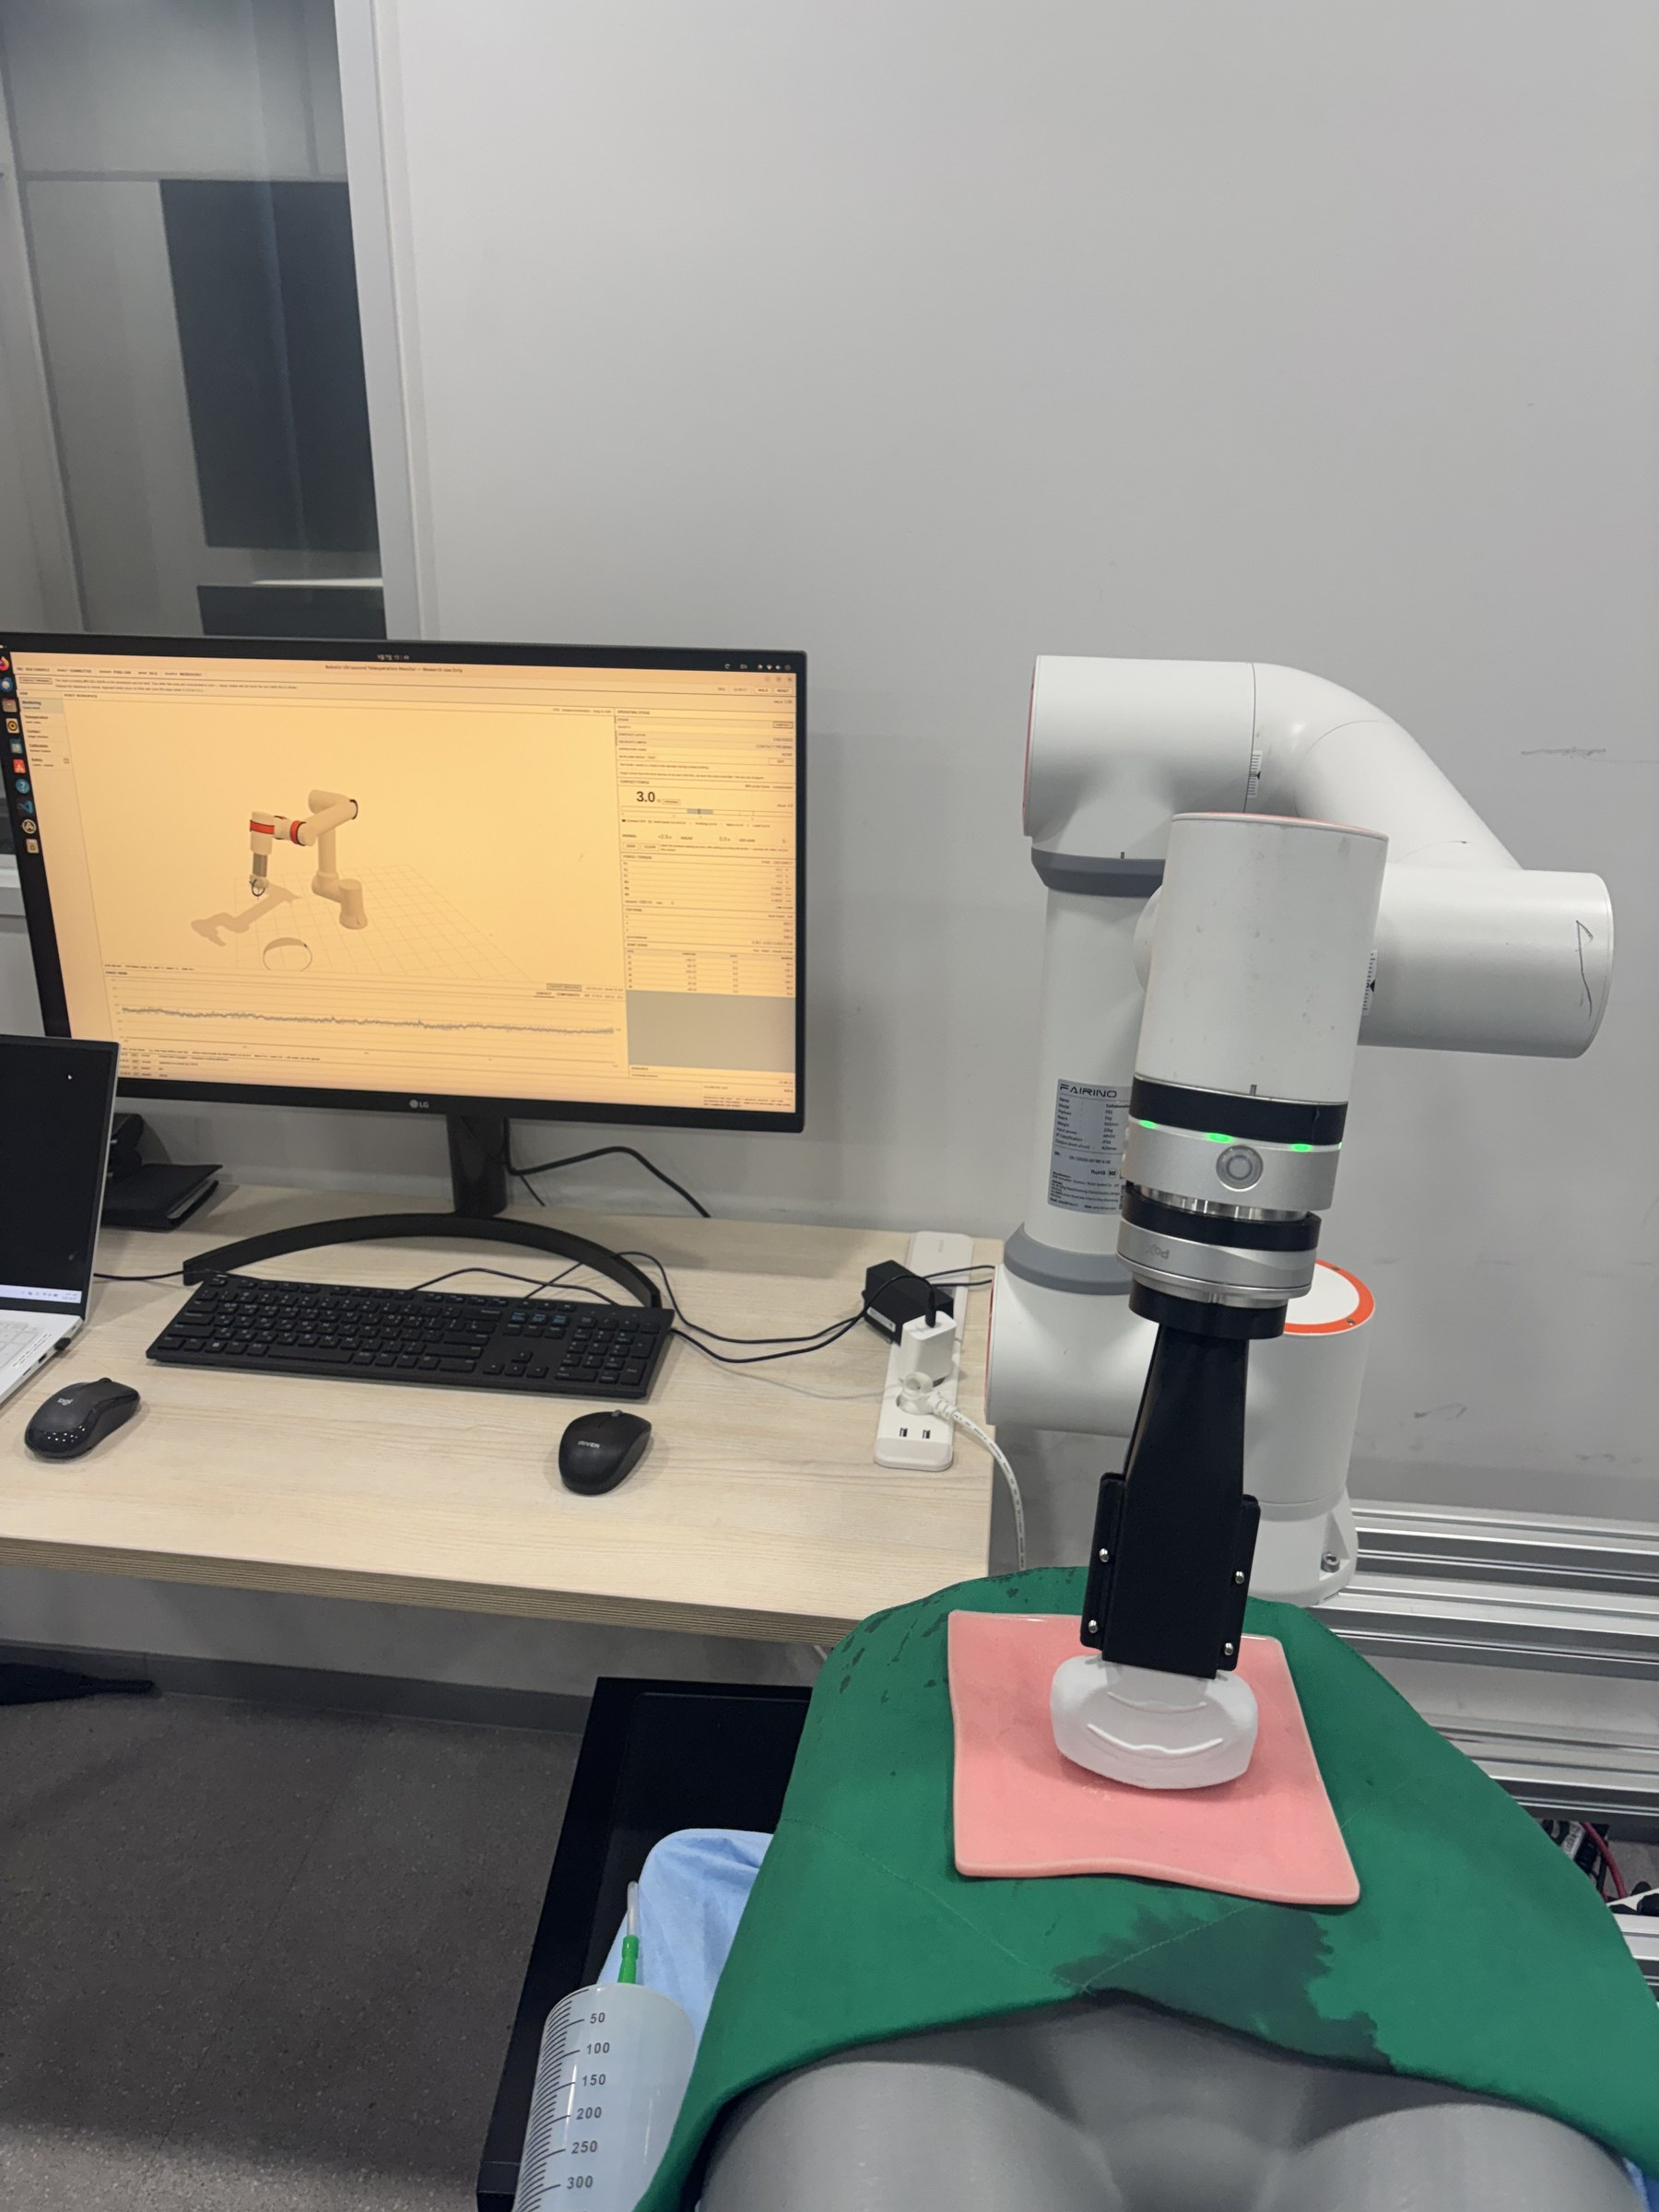
\includegraphics[width=0.315\textwidth]{figures/force_rig_syringe.jpg}\hfill
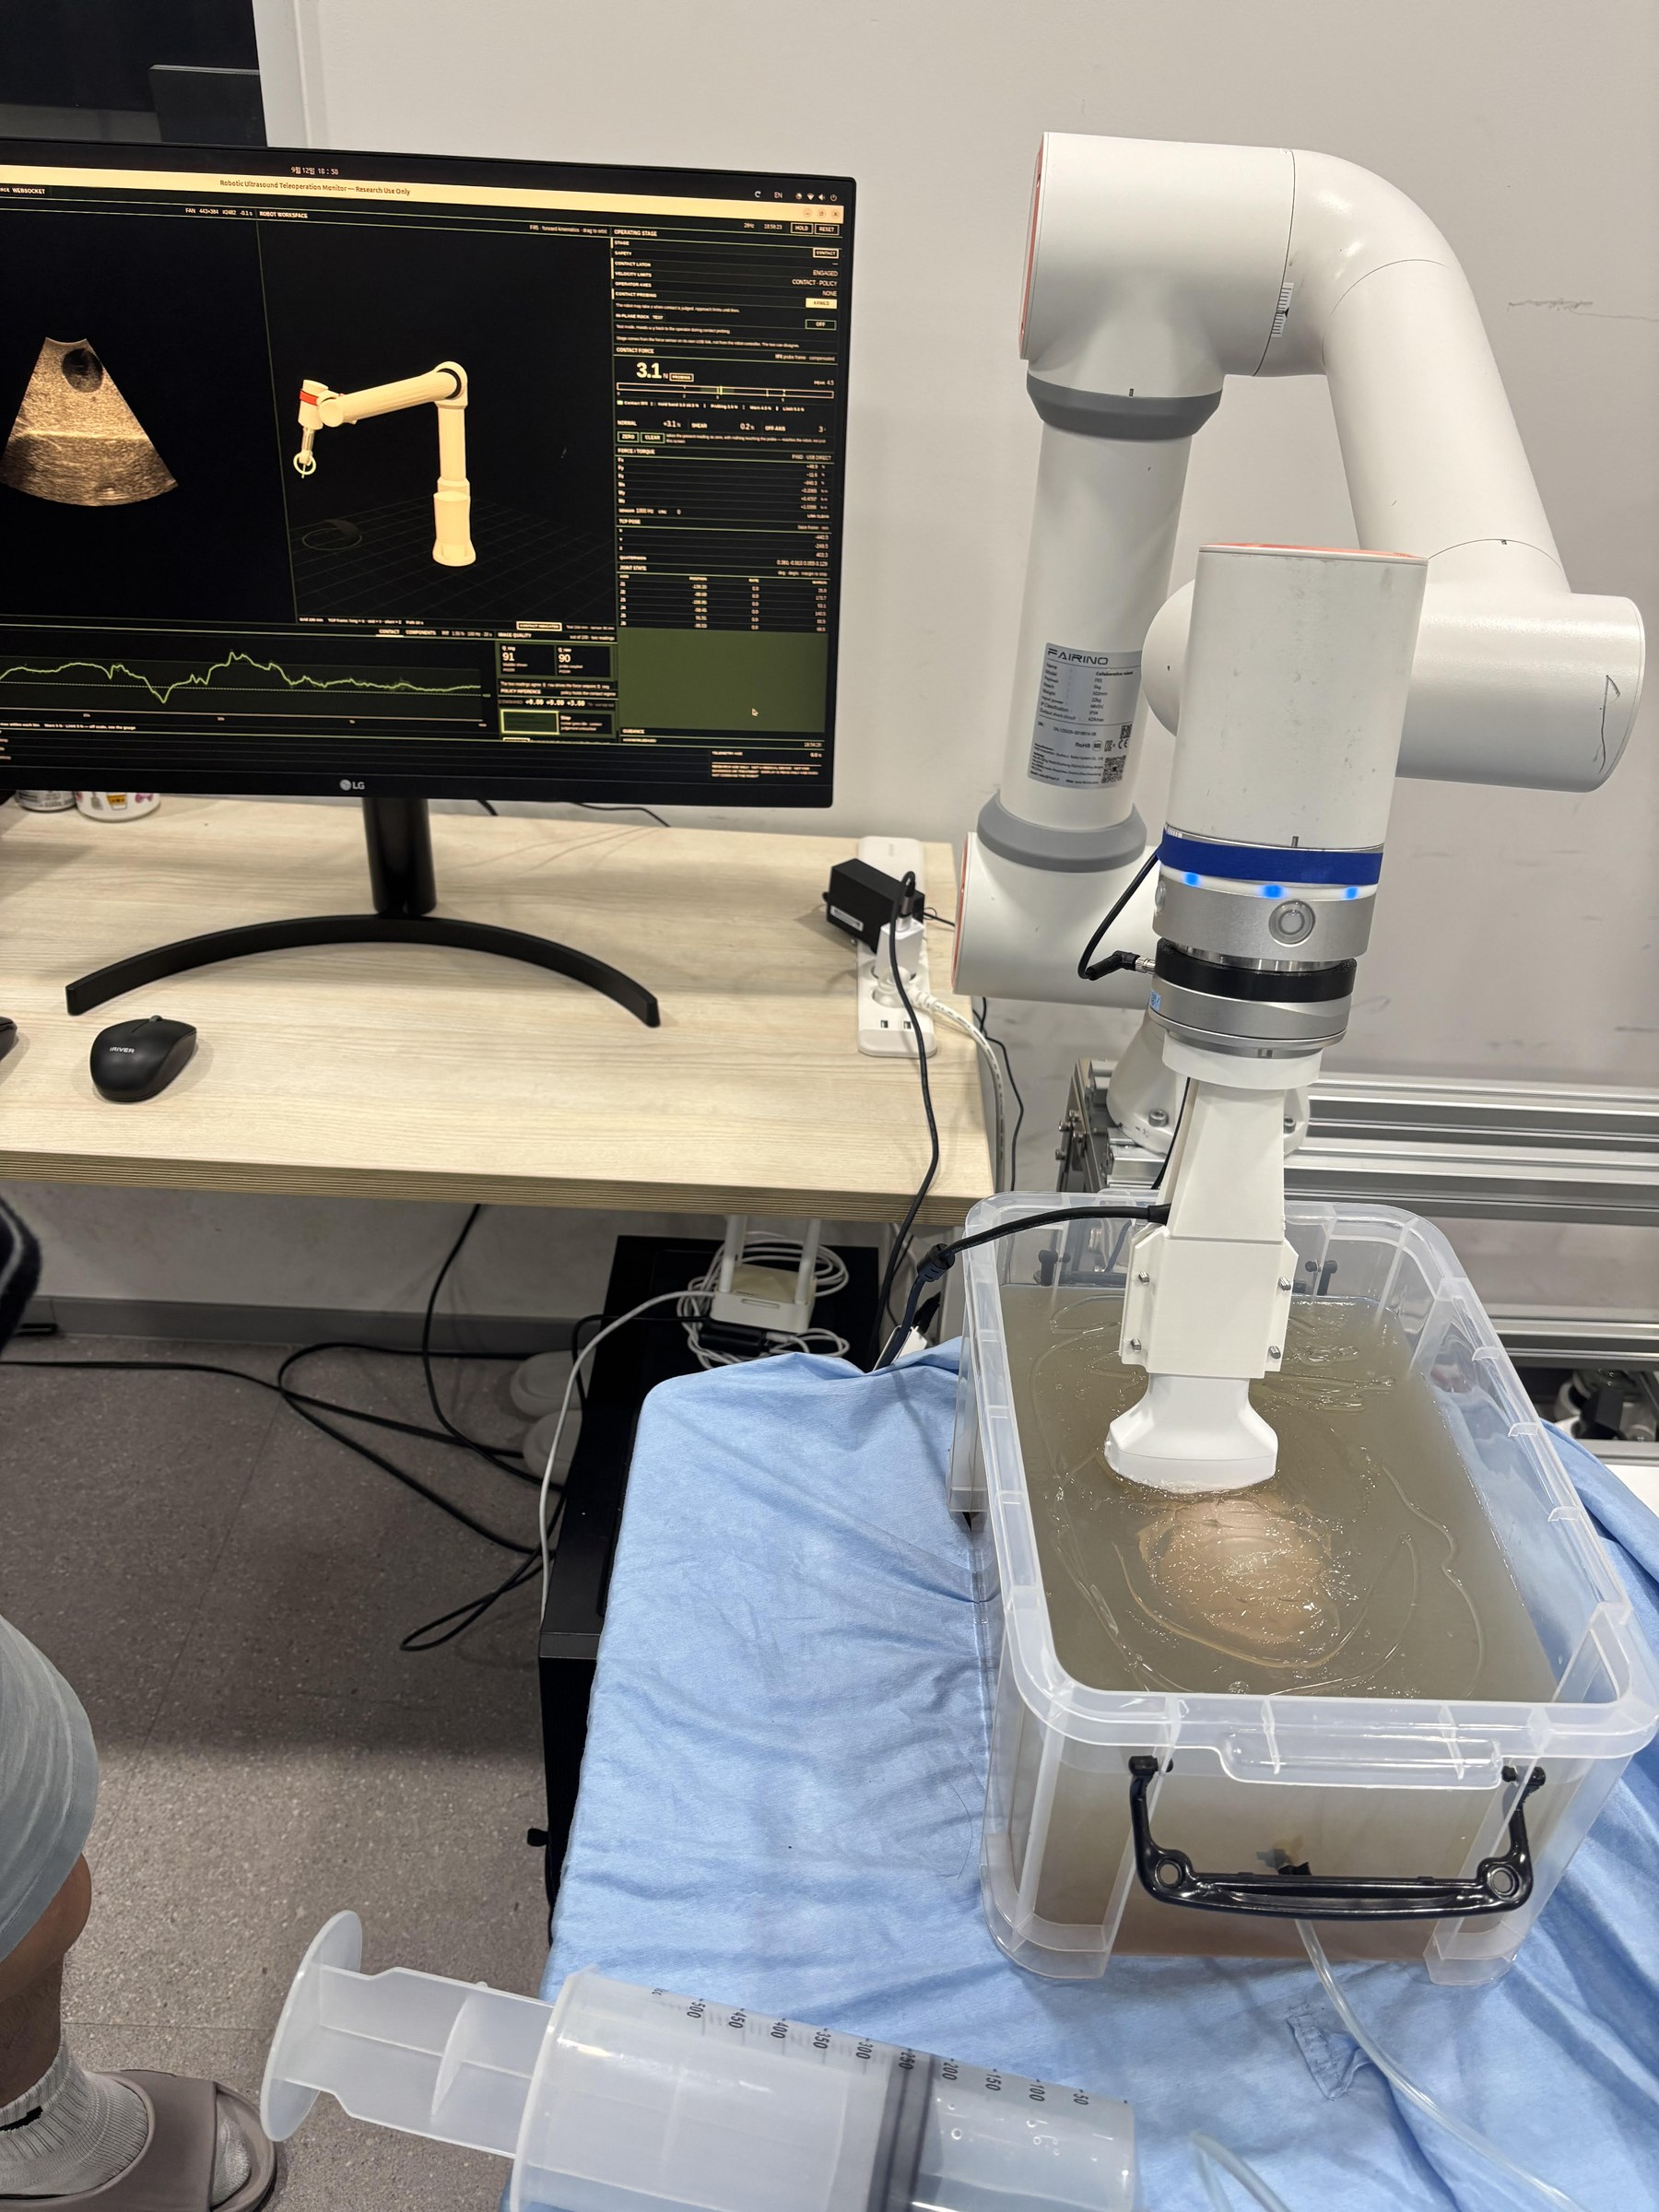
\includegraphics[width=0.315\textwidth]{figures/final_setup.jpg}\hfill
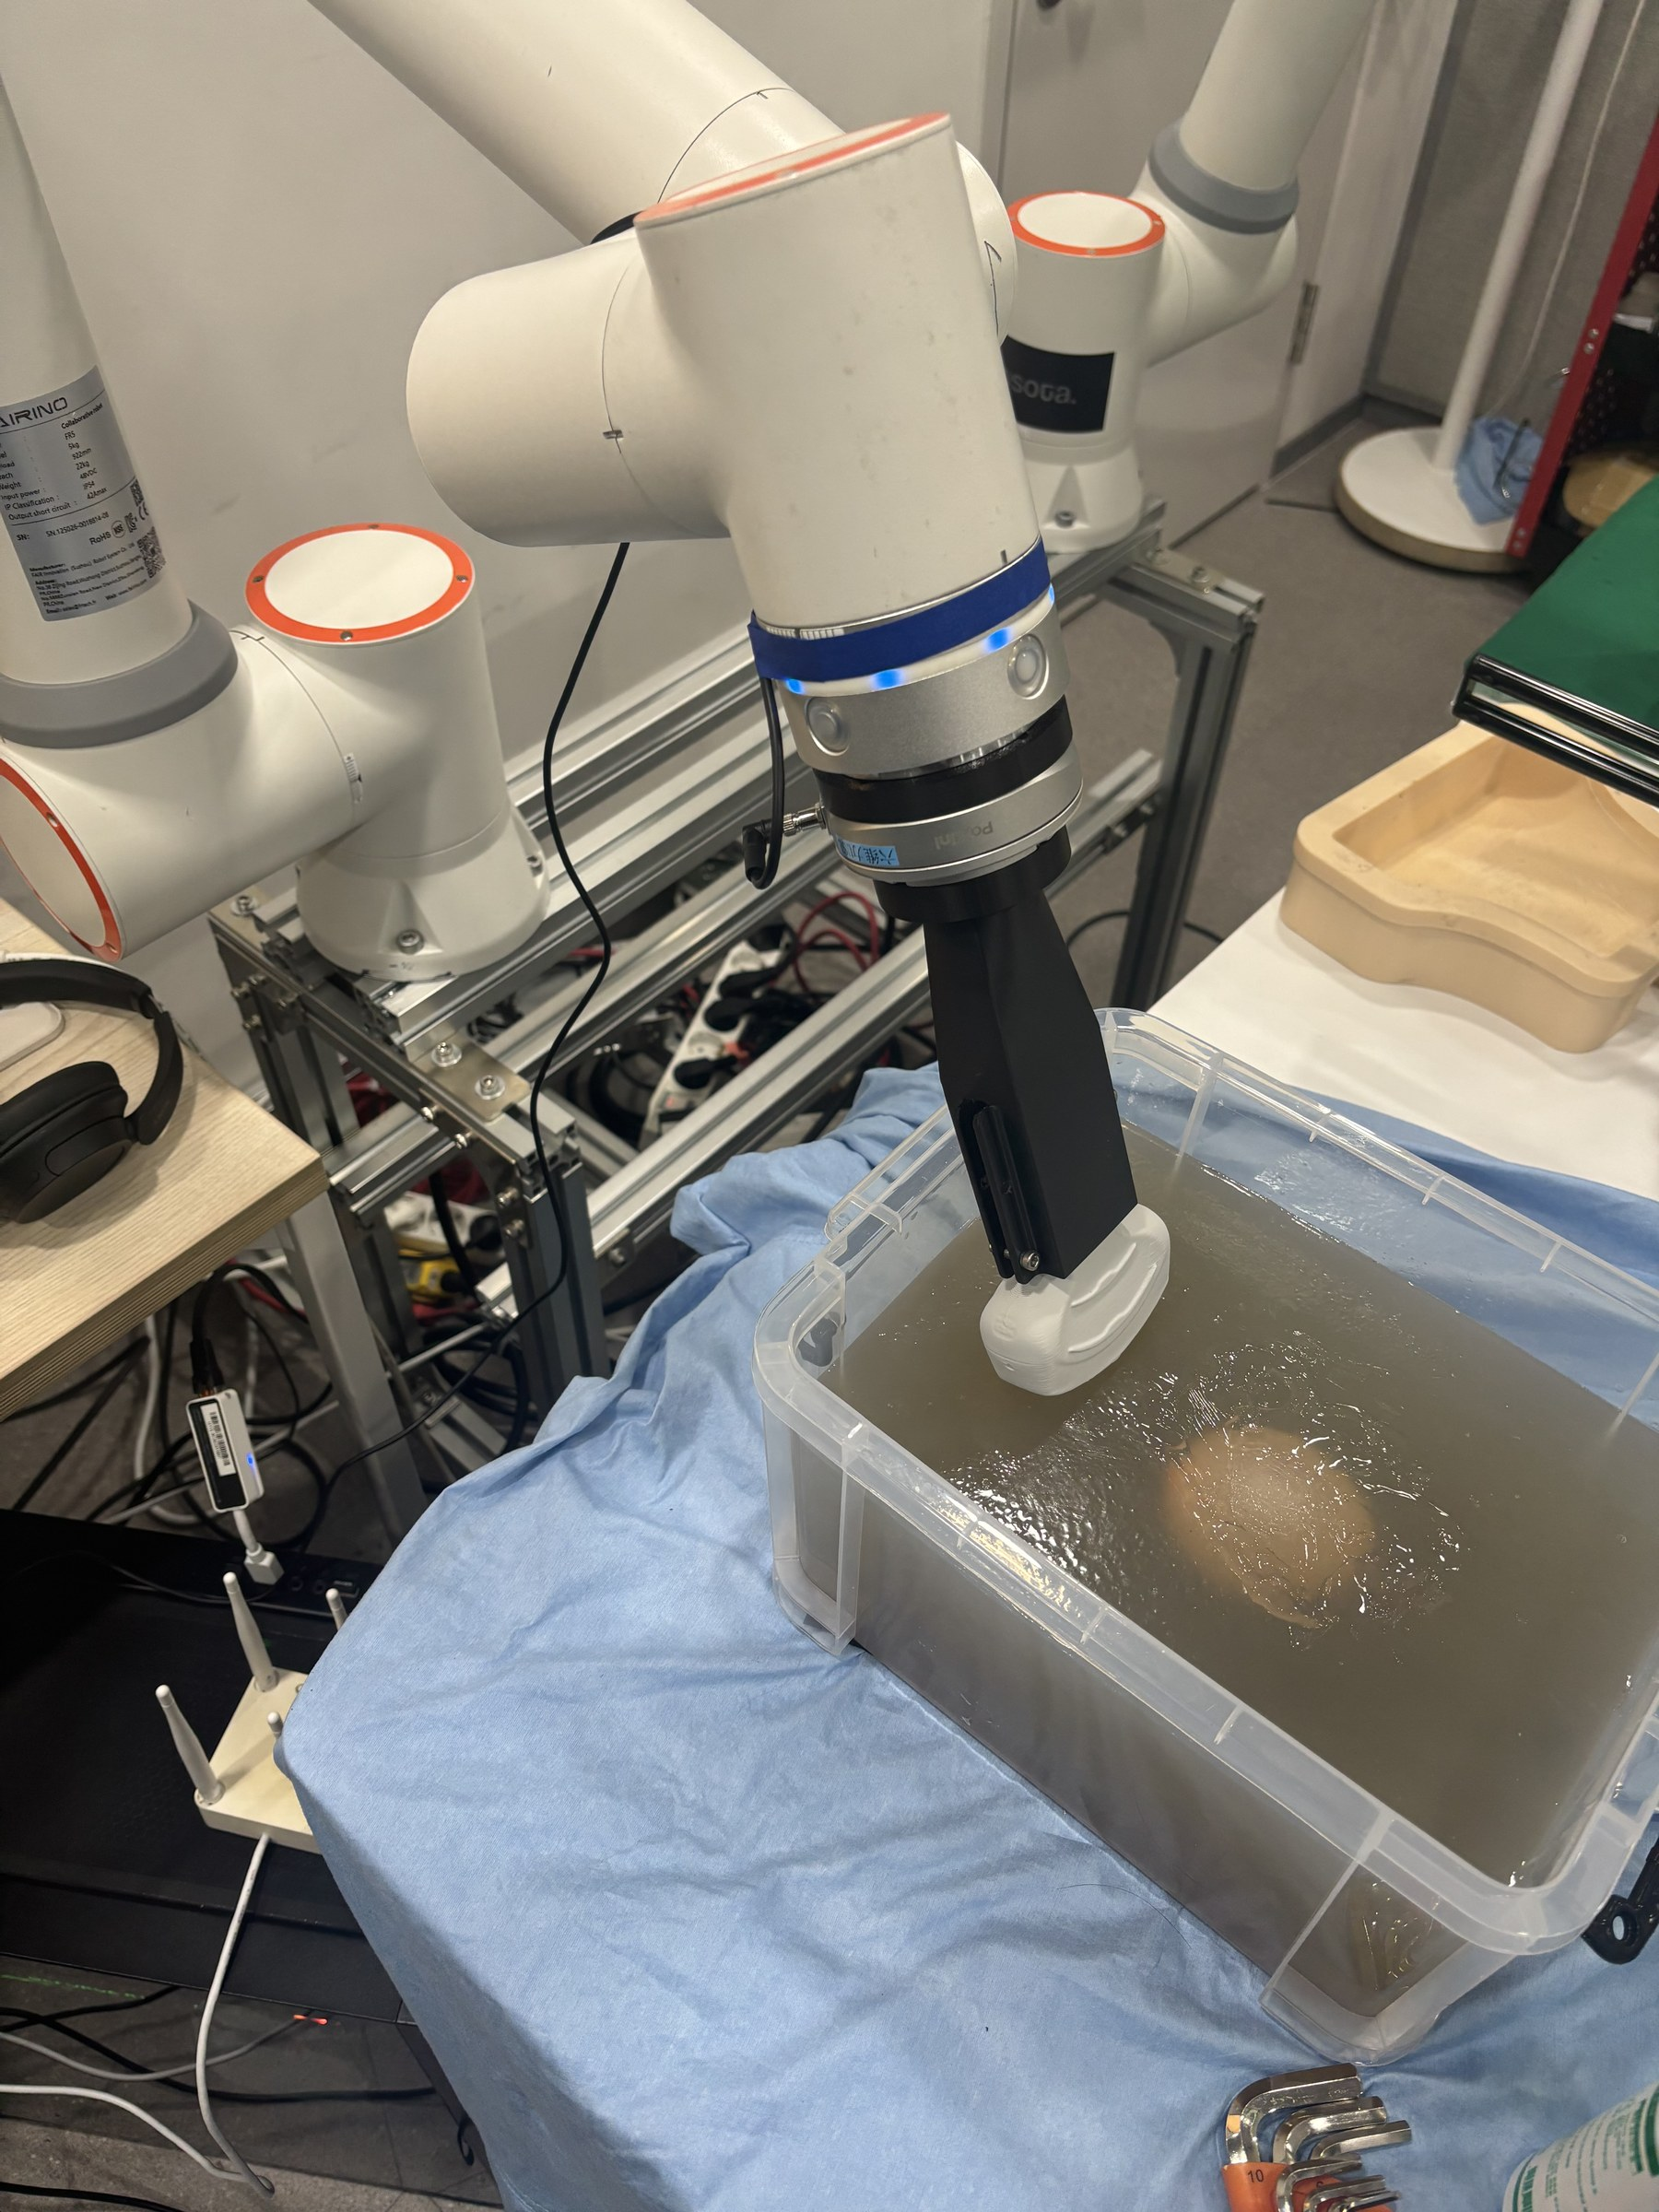
\includegraphics[width=0.315\textwidth]{figures/stiffness_measurement.jpg}
\caption{\textbf{The three benches.} (a) Force experiments: an inflatable air
tube inside a torso mannequin, inflated and deflated through a
\SI{500}{\milli\litre} syringe while the robot holds a commanded force.
(b) Final setup: the clinical probe on the gel bladder phantom in its water bath,
with the syringe line that fills and empties the lumen and the console the
operator watches. (c) Contact stiffness: a printed probe replica indents the gel
while force comes from the force/torque sensor and depth from forward
kinematics, so neither the scanner nor the control stack is involved (force
noise \SI{0.015}{\newton}, depth noise \SI{0.4}{\micro\metre}, indentation
steps about \SI{1}{\milli\metre}).}
\label{fig:benches}
\end{figure*}

\subsection{Pre-registered policy evaluation}

The evaluation is pre-registered. The primary endpoint is the acquisition
success rate, defined as reaching a diagnostic view within \SI{90}{\second} and
holding it for \SI{3}{\second}, where a diagnostic view requires simultaneously
a bladder mask area of at least \SI{8}{\percent} of the frame, a largest
connected component of at least \SI{80}{\percent} of the mask, and a lateral
centroid within \num{0.30} of the frame centre. Neither $\hat Q$ nor
$Q_\mathrm{raw}$ is a primary endpoint: the first is the policy's own objective
and would be circular, and the second measures coupling rather than anatomy.

Each episode begins from a teleoperated approach to a starting pose in which the
bladder is not visible although coupling is good (area below \SI{2}{\percent}
with $Q_\mathrm{raw} \ge \num{0.6}$); the operator then releases the stylus and
starts inference from the console. Conditions are hold (no command), placebo,
policy, and optionally expert teleoperation as an upper bound. The placebo is
pre-registered as motion of the same magnitude and duration as the policy's with
the direction destroyed: the axes of the selected rotation command are shuffled
and the signs flipped, so the multiset of command magnitudes is preserved
exactly. Condition order is randomised within each starting pose and the
operator is blind to the condition. The primary analysis is a paired McNemar
exact test of policy against placebo with bootstrap confidence intervals, with
Wilson intervals for proportions and a log rank test on acquisition time as a
secondary analysis. A blinded human read of the last five seconds of each
episode by two readers on a five point scale, with weighted $\kappa$, is
reported alongside the automatic criterion.

The pre-registration also fixes what would refute the claim: if policy is
indistinguishable from placebo, the direction selection contributes nothing; if
the safety indicators are poor, the system is unusable regardless of success
rate.



\section{Results}
\label{sec:results}


\begin{figure*}[t]
\centering
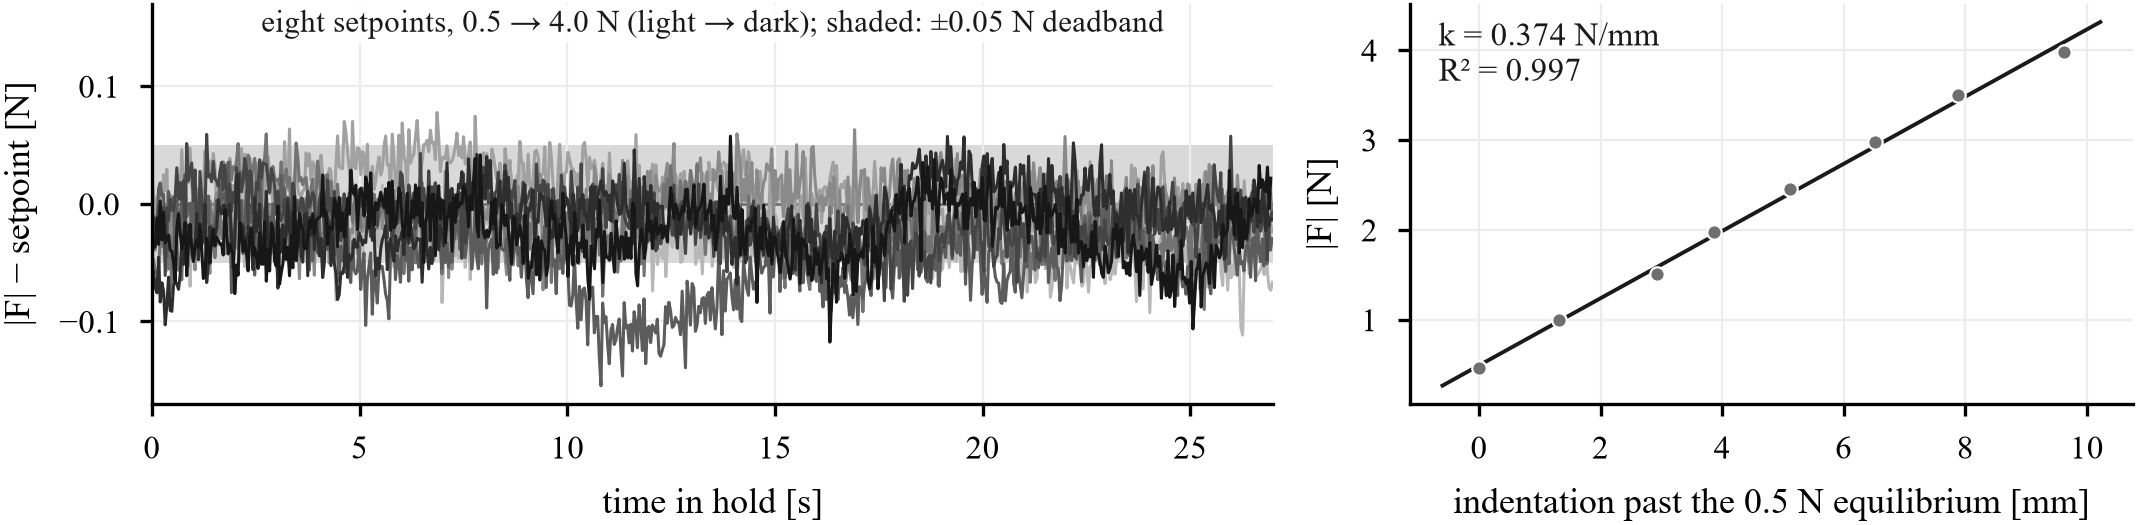
\includegraphics[width=\textwidth]{figures/force_hold_bands.png}
\caption{\textbf{Force hold at eight set points.} Left: error from the commanded
force during the scored part of each hold, all eight set points from
\SIrange{0.5}{4.0}{\newton} overlaid (light to dark), with the
\SI{\pm 0.05}{\newton} dead band shaded; the first \SI{3}{\second} of each hold
are discarded and the traces are \SI{1}{\kilo\hertz} samples pooled over two
independently calibrated sessions. Right: the equilibrium force against
indentation past the \SI{0.5}{\newton} point, whose slope is the phantom
stiffness used in the time constant above.}
\label{fig:hold}
\end{figure*}

\subsection{Force regulation}

Fig.~\ref{fig:hold} shows every hold as an error trace against its own set
point. Across the 16 holds the standard deviation of the held force is
\SI{0.028}{\newton} on average and \SI{0.073}{\newton} at worst, every hold sits
inside the \SI{\pm 0.05}{\newton} dead band, and the worst mean error is
\SI{0.049}{\newton} (Table~\ref{tab:force}). Relative error falls from
\SI{6.3}{\percent} at \SI{0.5}{\newton} to \SIrange{0.8}{1.4}{\percent} above
\SI{3}{\newton}, and the two independently calibrated sessions agree to within
\SI{0.047}{\newton}, which is the reproducibility of the whole chain including
recalibration.

Under volume disturbance the loop behaves as its time constant predicts. Syringe
steps arrive with a median spacing of \SI{4.6}{\second} and the force peak
occurs \SI{3.1}{\second} after a step, while the dead band re-entry time is
about \SI{35}{\second}. Consequently the regulator does not reduce the peak
(\SI{0.83}{\newton} against \SI{0.74}{\newton} with the loop disabled on
injection), but it does change everything after the peak: the probe travels
\SI{0.17}{\milli\metre} (IQR \numrange{0.13}{0.24}) against
\SI{0.01}{\milli\metre}, the post peak return rate rises to
\SI{0.23}{\newton\per\second} from \SI{0.13}{\newton\per\second}
($p < \num{0.001}$, $n = 70$ events per arm), and the residual deviation at the
next step falls to \SI{0.28}{\newton} from \SI{0.38}{\newton} ($p = \num{0.011}$).
We report this as a bounded claim: on this phantom the loop recovers from
disturbances but does not attenuate their peaks, and closing that gap requires a
faster loop than the limit cycle permits.

The hard limit was exercised rather than assumed. In the two runs at the
\SI{4.0}{\newton} set point the disturbance drove the force to
\SI{5.38}{\newton} and the \SI{5}{\newton} retreat fired; in all other runs the
peak stayed below the warning line.

\begin{table}[t]
\caption{\textbf{Force hold on the air tube mannequin phantom.} Pooled over
two independently calibrated sessions, \SI{30}{\second} per hold, first
\SI{3}{\second} discarded, \SI{1}{\kilo\hertz} sampling.}
\label{tab:force}
\centering
\begin{tabular}{ccccc}
\toprule
Target [N] & SD [N] & Mean error [N] & In band [\%] & Peak [N] \\
\midrule
0.5 & 0.023 & $-0.017$ & 88.9 & 0.60 \\
1.0 & 0.022 & $-0.013$ & 83.9 & 1.10 \\
1.5 & 0.022 & $-0.012$ & 94.1 & 1.57 \\
2.0 & 0.026 & $-0.016$ & 89.9 & 2.09 \\
2.5 & 0.029 & $-0.031$ & 72.9 & 2.59 \\
3.0 & 0.026 & $-0.015$ & 89.7 & 3.10 \\
3.5 & 0.025 & $-0.008$ & 93.7 & 3.59 \\
4.0 & 0.049 & $-0.025$ & 82.9 & 4.36 \\
\bottomrule
\end{tabular}
\end{table}

\subsection{Demonstration quality}

Table~\ref{tab:imu} summarises the comparison that justifies the demonstration
route: six axis fusion on the host against the on chip nine axis rotation
vector, on the same recordings, next to the robot.

\begin{table}[t]
\caption{\textbf{Probe orientation against robot forward kinematics.} Host side
six axis fusion against the on chip nine axis rotation vector, same recordings,
near the robot.}
\label{tab:imu}
\centering
\begin{tabular}{lcc}
\toprule
 & Six axis & Nine axis \\
\midrule
Axial rotation RMS [\si{\degree}]        & 1.95 & 11.23 \\
Tilt $x$ RMS [\si{\degree}]              & 1.14 & 6.17 \\
Tilt $y$ RMS [\si{\degree}]              & 0.73 & 3.98 \\
Static alignment residual [\si{\degree}] & 0.81 & 6.68 \\
Axial drift [\si{\degree\per\minute}]    & 0.23 & 8.29 \\
\bottomrule
\end{tabular}
\end{table}

\subsection{What the policy learned}

Rotation is learned and translation is not. Against label dispersions of
\SI{14.5}{\milli\metre} and \SI{13.4}{\milli\metre} in the lateral and
elevational translation axes, the model's mean absolute errors are
\SI{12.2}{\milli\metre} and \SI{7.0}{\milli\metre}, which is the accuracy of
predicting a constant; against a rotation label dispersion of
\SI{0.96}{\degree} the errors are \SIrange{0.36}{0.66}{\degree}. This is the
empirical reason the deployed policy commands rotation only.

\subsection{Closed loop policy}

\TODO{Main result: success rate per condition with Wilson intervals, the paired
McNemar comparison, acquisition time, and behaviour while the dynamic phantom
volume changes. As of this draft, 4 of 18 pilot episodes have been run and none
reached the success criterion.}

\begin{figure}[t]
\centering
% \includegraphics[width=\linewidth]{fig3_results.pdf}
\figspace{38mm}
\caption{\textbf{Closed loop behaviour on the dynamic bladder phantom.}
\TODO{caption once the runs are complete}}
\label{fig:results}
\end{figure}

\subsection{The quality head learns magnitude, not direction}
\label{sec:negative}

Candidate selection, equation~\eqref{eq:select}, is where image information is
supposed to enter, and it is where the current model fails in an instructive
way. We measure the head directly with a mirror test: each candidate chunk is
scored against a copy of itself with the elevational tilt sign flipped, and the
head is asked which of the two is better. The trained head prefers the correct
direction on \SI{52.4}{\percent} of held out observations, against a chance
level of \SI{50}{\percent}, while it prefers the larger of two otherwise
identical motions on \SI{70.1}{\percent}. Retraining the head on an area
weighted quality label raises the label fit from $R^2 = \num{0.081}$ to
\num{0.536} and the action effect correlation from \num{-0.035} to
\num{+0.196}, yet moves the mirror test only to \SI{56.3}{\percent}. The two
apparently improved numbers are explained by magnitude: in freehand data the
size of a motion is correlated with the size of the resulting area change, so a
head that has learned only ``larger is better'' improves on both.

The consequence in closed loop is a policy that tilts steadily in one
elevational direction rather than searching. On 480 held out observations the
decoder proposes elevational tilt in both directions in equal proportion
(\SI{52}{\percent} positive), matching the demonstration labels
(\SI{50.4}{\percent} positive), but ranking those candidates by $\hat Q$ selects
the negative direction in \SI{84}{\percent} of observations, and the candidate
mean is uncorrelated with the demonstrated label ($\rho = \num{-0.04}$).
Lowering the mode consistency bonus makes the lock stronger rather than weaker
(\SI{78}{\percent} at $\gamma = \num{0.2}$, \SI{84}{\percent} at
$\gamma = 0$), which places the bias in the quality head and not in the
selection prior. The retrained head is worse in exactly this sense: it selects
one direction in \SI{91}{\percent} of observations.

Part of the explanation is the objective itself. The head was trained to predict
the original $Q_\mathrm{seg}$, whose span between ``no bladder'' and ``bladder
perfectly captured'' is \num{0.06} (Sec.~\ref{sec:percep}), while the span
between a small and a large motion in the same data is larger than that. Given
that target, a head that reports motion magnitude is not a bug but the best
available fit.

We report this because it is also a property of the data rather than only of the
implementation. In demonstrations recorded by a sonographer who is already
looking at the screen, the direction of motion is confounded with the operator's
decision; the marginal rank correlation between elevational tilt and the
subsequent area weighted quality change is $\rho = \num{+0.10}$ on the training
split and $\num{-0.03}$ on test, which is below what candidate ranking can use,
and of the opposite sign to the direction the head prefers. Direction requires
interventional data: sweeps executed by the robot itself, labelled by forward
kinematics, in which the direction is imposed rather than chosen. As an interim
control we also evaluate a condition that replaces the learned ranking with
measured hill climbing on $Q_\mathrm{seg}$, which needs no new data but pays for
every decision with probe motion.

\section{Limitations}
\label{sec:limits}

\begin{itemize}
\item \textbf{One phantom, one operator.} All demonstrations come from a single
bladder phantom, so validation and test splits measure reproducibility rather
than generalisation, and no clinical data are used. Clinical recording is
planned as non-interventional observation with no robot and no force control
applied to subjects.
\item \textbf{Direction is not learned} (Sec.~\ref{sec:negative}). The system
maintains contact and image quality; it does not yet decide where to look.
\item \textbf{Peaks are not attenuated.} The force loop recovers from volume
disturbances but does not reduce their peaks, because its time constant
(\SI{12}{\second}) is far longer than the disturbance spacing
(\SI{4.6}{\second}); faster gains reintroduce a limit cycle.
\item \textbf{A sub newton force offset remains.} The scale factor is accurate
to \SI{2}{\percent}, but a bias of \SI{-0.29}{\newton} and an attitude dependent
compensation residual of the same order are not removed.
\item \textbf{The orientation accuracy and the demonstration corpus come from
different probes.} The bench characterisation against robot kinematics used an
instrumented probe on a different scanner from the one used for the phantom
demonstrations, and the clamp geometry differs; the transfer of the orientation
figures between the two has not been measured.
\item \textbf{Sign convention of two axes.} The axis assignment of the sensor to
probe rotation is certain; the signs of the lateral and elevational rows are
supported by conflicting evidence.
\item \textbf{Vertical centring is unreachable.} At the depth setting used, the
target lies in the near field and cannot be brought to the vertical centre of
the frame by any probe motion, so a servo target defined in frame coordinates is
infeasible in that axis.
\item \textbf{Presence errors dominate segmentation error.} Boundaries are
accurate, but the network still puts a mask on about half of audited empty
frames.
\item \textbf{Force labels were never supervised.} The force head and the
feasibility and risk terms received no gradient, because the freehand
demonstrations carry no valid force channel.
\end{itemize}

\section{Conclusion}

We described an ultrasound robot for the bladder monitoring task of HoLEP
morcellation, in which contact force is regulated inside a verified envelope and
the image objective is learned from demonstrations that were never collected on
the robot. The demonstration route is validated end to end: six axis probe
mounted inertial sensing recovers rotation to \SI{2.50}{\degree} against robot
kinematics, the two streams are aligned to a measured \SI{200}{\milli\second},
and the resulting chunks train an action chunking policy with a predicted
quality head. \TODO{closing sentence once the closed loop results are in.} The
negative result on direction learning identifies precisely which data the next
iteration needs, and it is data this platform can now collect by itself.

\bibliographystyle{IEEEtran}
\bibliography{refs}

\balance
\end{document}
